\begin{homeworkProblem}

\textbf{Bivariate Standard Normal Distribution:} Implement a Gibbs sampler to generate samples from a bivariate standard normal distribution with correlation $\rho=0.6,-0.6$.

\solution

Suppose that the correlation of the bivariate standard normal distribution is $\rho\in(-1,1)$, which means that the covariance matrix is $\Sigma=\begin{bmatrix}
    1 & \rho \\
    \rho & 1
\end{bmatrix}$. Thus the joint PDF is
$$f_{X,Y}(x,y)=\dfrac{1}{2\pi\sqrt{1-\rho^2}}e^{-\frac{x^2-2\rho xy+y^2}{2(1-\rho^2)}}$$
So we can derive that the conditional PDF of $X$ given $Y=y$ is
$$f_{X|Y=y}(x|Y=y)\propto e^{-\frac{(x-\rho y)^2}{2(1-\rho^2)}}\sim\N(\rho y,1-\rho^2)$$
Similarly, the conditional PDF of $Y$ given $X=x$ is
$$f_{Y|X=x}(y|X=x)\propto e^{-\frac{(y-\rho x)^2}{2(1-\rho^2)}}\sim\N(\rho x,1-\rho^2)$$
Then we can apply the Gibbs sampler to generate samples from the bivariate standard normal distribution with correlation $\rho=0.6,-0.6$ in 1000000 samples, and the burn in is set to be 10000 samples. The results are as follows:

\begin{figure}[h]
    \centering
    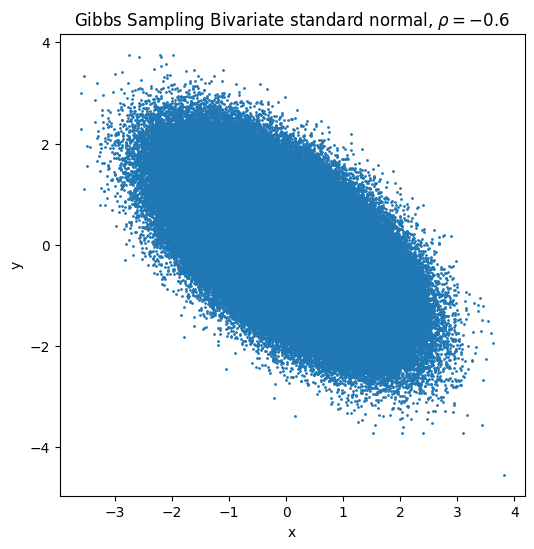
\includegraphics[width=0.48\textwidth]{./figure/p7/-0.6.png}
    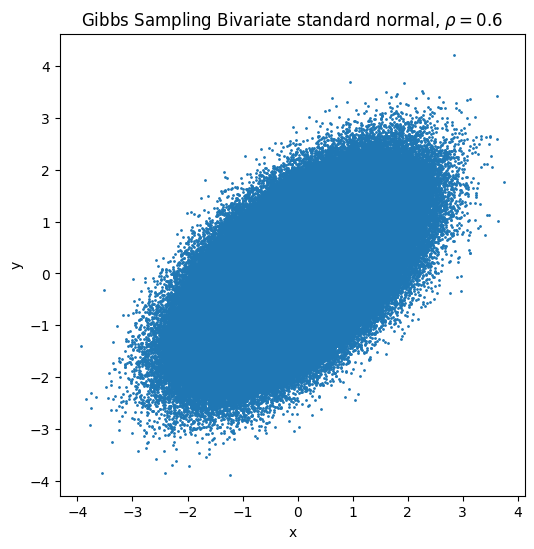
\includegraphics[width=0.48\textwidth]{./figure/p7/0.6.png}
\end{figure}

\end{homeworkProblem}

\newpage